% This file contains the templates for the first few pages of the thesis including 
% 1. Title page
% 2. Dedication
% 3. Dissertation approval
% 4. Declaration of authorship
% 5. Abstract


%   1. TITLE
\newcommand{\titlePage}{

% No page number
\thispagestyle{empty}
\begin{center}

% thesis title
\vspace*{15px}
{\Huge\bfseries \thesisTitle}\\[1.0cm] 

% submitted in partial fulfillment etc.
\textit{Submitted in partial fulfillment of the requirements\\[0.2cm] of the degree of\\[0.2cm] \degree}\\[2.0cm]
 
% author
\textit{by}\\[0.2cm]
\authorName \\[0.2cm] (\textit{Roll no.} \rollNo) \\[2.0cm]

% supervisor
\textit{Supervisor:}\\[0.2cm]
% or
% \textit{under the supervision of}\\[0.2cm]
\supervisorOne \\[2.0cm]

% iit-b logo

\includegraphics[width=0.25\textwidth]{Figures/iitb_logo.jpg}

\vspace*{10px}

% department and college
\dept\\[0.2cm]
\college\\[0.2cm]

% year
\currentyear\\[4cm] 

\end{center}

\clearpage
}


%   3. DISSERTATION APPROVAL

\newcommand{\approval}{
% if you use a dedication, then use a page number with the plain page style
\thispagestyle{plain}
% else, use no page number with the empty page style
%\thispagestyle{empty}


\begin{figure}[h]
\centering
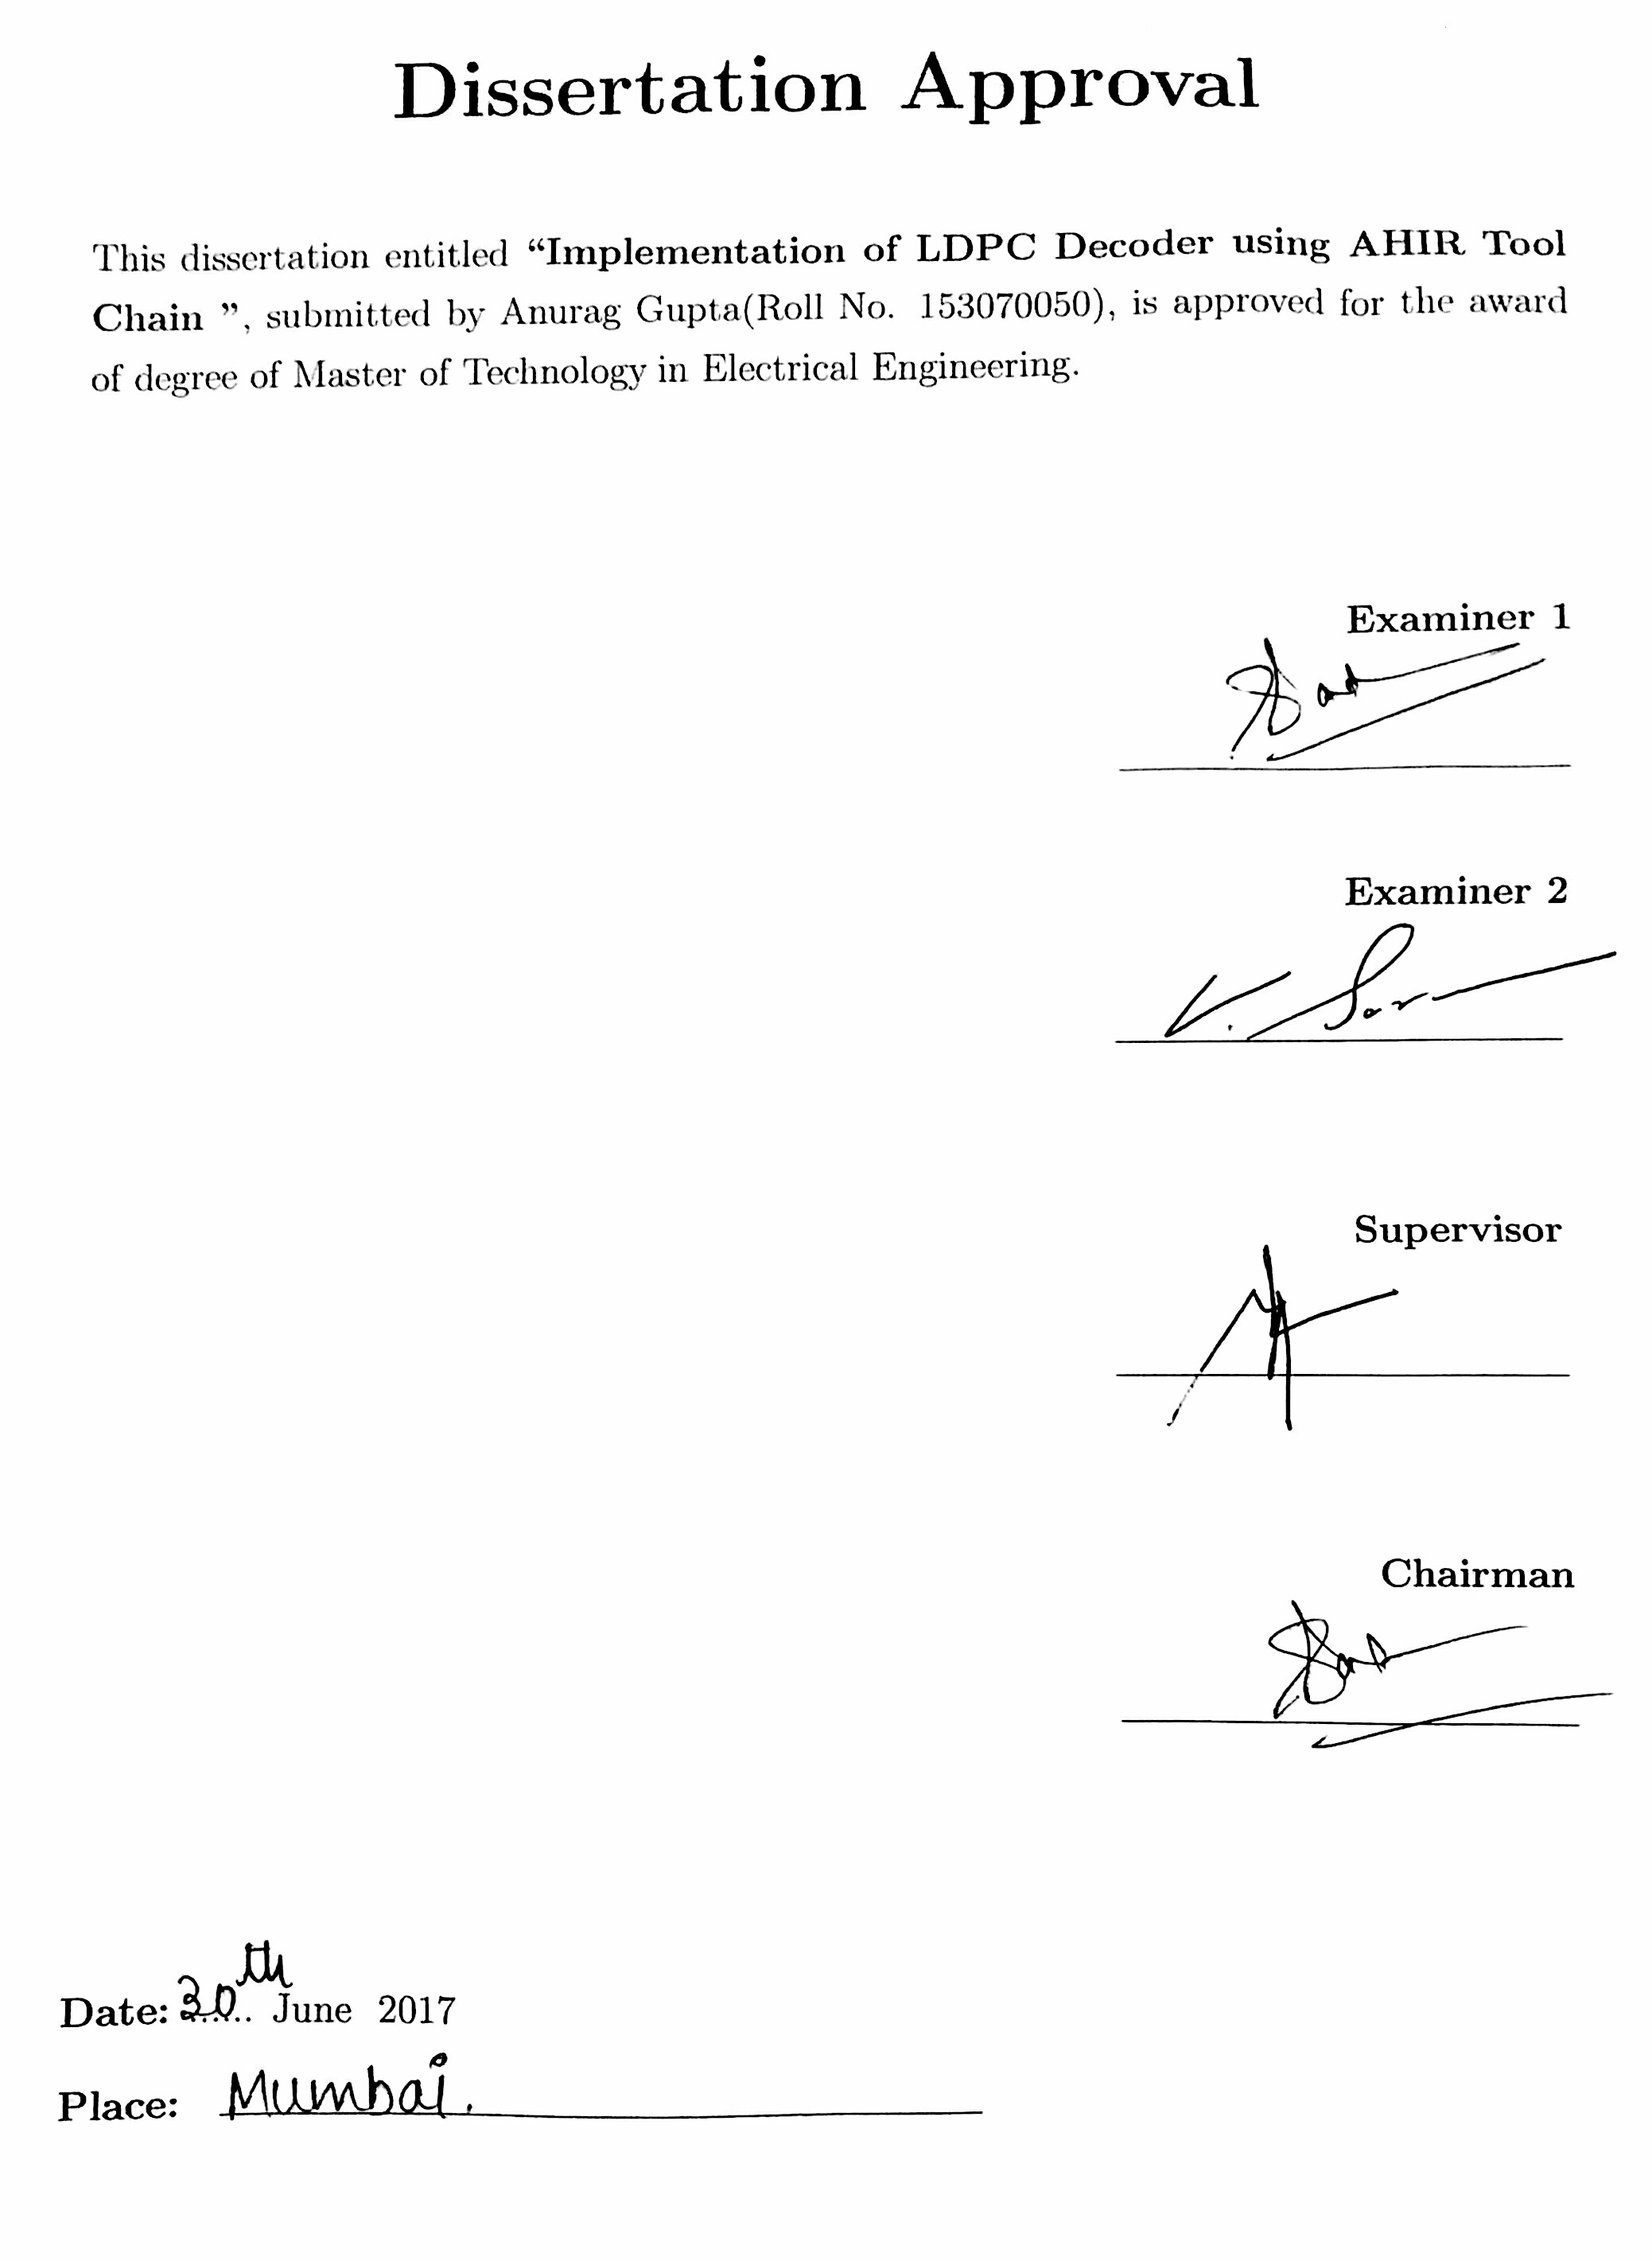
\includegraphics[height=25cm,width=16cm]{11.jpg}
\end{figure}
\clearpage 
\clearpage
}

%   4. DECLARATION OF AUTHORSHIP
\newcommand{\authorship}{
\thispagestyle{plain}

\begin{figure}
\centering
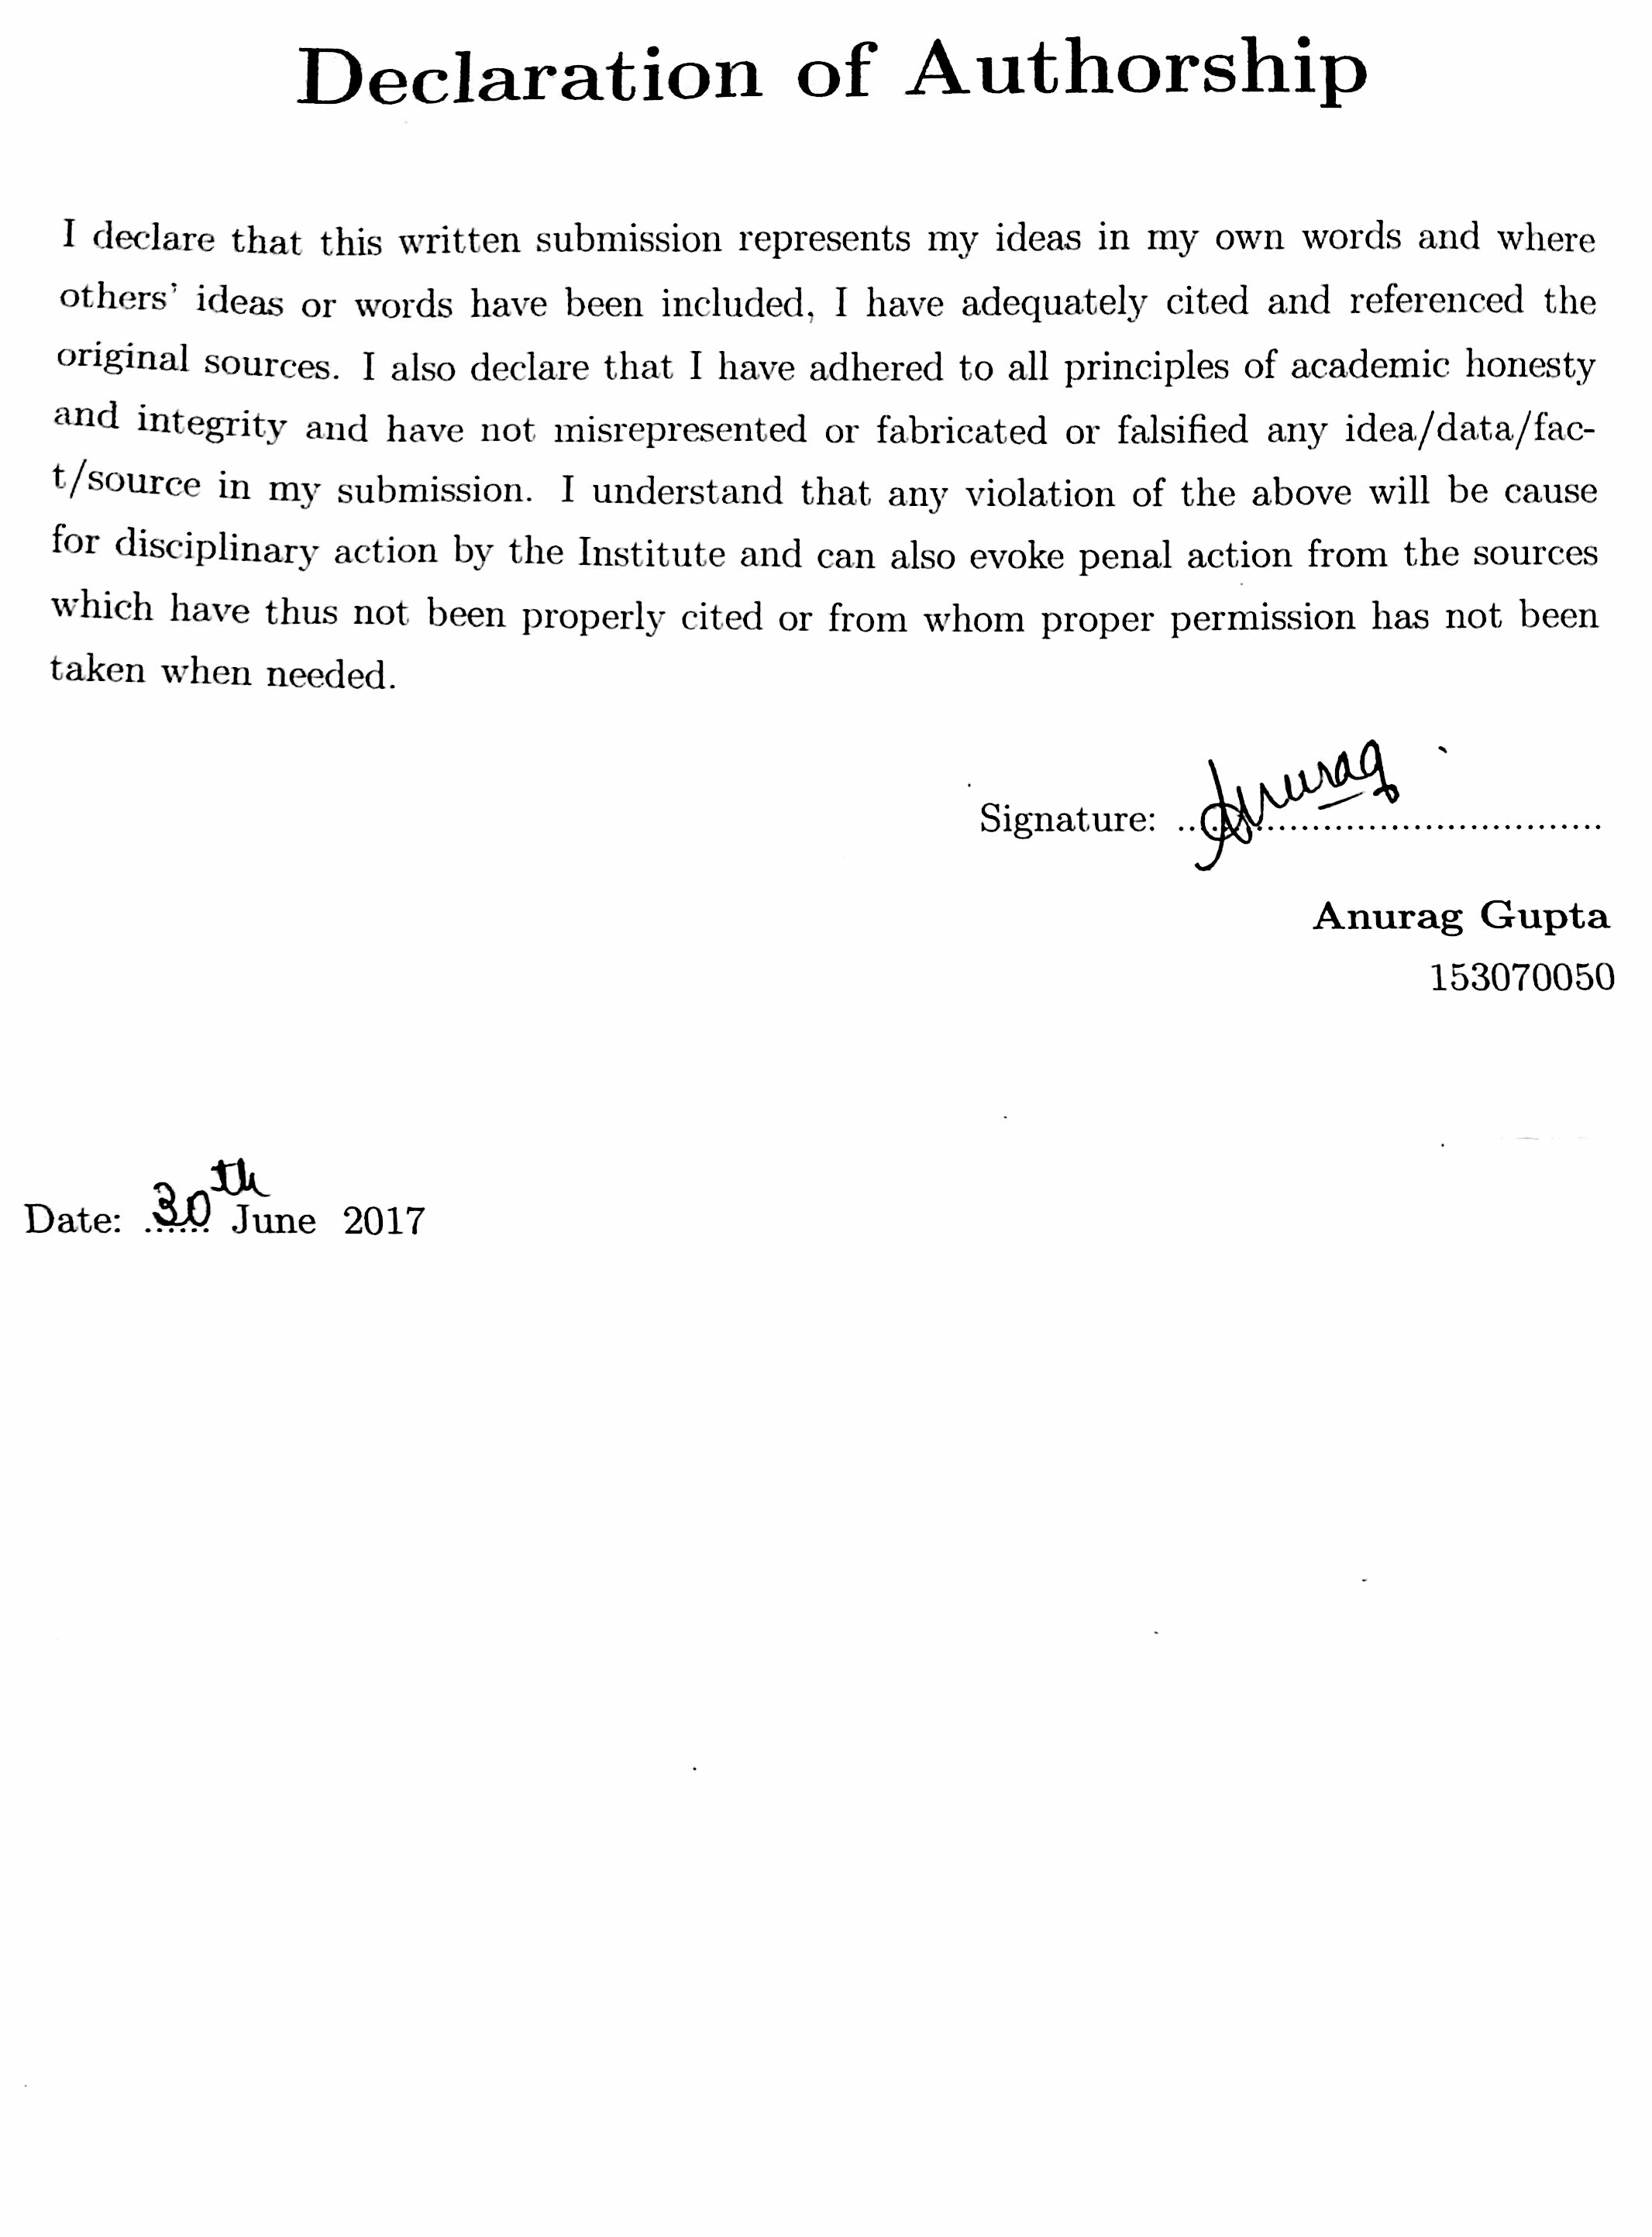
\includegraphics[height=25cm,width=16cm]{22.jpg}
\end{figure}
\clearpage 
}


%   2. DEDICATION
\newcommand{\dedication}{
\thispagestyle{empty}
\vspace*{150px}
\begin{center}\large{\textit{To Maa Papa \& Tannu}} \\


\end{center}

\clearpage
}


%   5. ABSTRACT
\newcommand{\abstractpage}{
\thispagestyle{plain}

% header-type text for the abstract - optional
%\small {\noindent\authorName/ \supervisorOne{ }(Supervisor): \textbf{``\thesisTitle"}, \textit{Master of Technology Dissertation}, \dept, \college, \currentmonth { } \currentyear.}\\[0.0cm]
%\HRule\\[0.2cm]


\vspace*{10px}

\begin{center}{\huge{\textit {Abstract}}\par}\end{center}

\vspace*{10px}

% Abstract text - Type abstract here
\noindent We have investigated performance of Min Sum decoder for  decoding Low Density Parity Check (LDPC) codes using AHIR tool chain. AHIR is an open source tool - used for High Level Synthesis (HLS),  developed at IIT Bombay. \\
Construction of Low Density Parity Check (LDPC) codes involves generation of Low Density Parity Check (LDPC) matrices. We generated Gallager, Quasi-Cyclic (QC) and Neal-Mckey class of matrices. The focus was to use the construction for storage systems. \\
For Low Density Parity Check (LDPC) codes some decoding algorithms can achieve error-correction performance very close to the Shannon limit. We have characterised Sum Product algorithm and Min Sum algorithm in C to decode the code block. The algorithms are written in C so that the description can be converted into hardware via High Level Synthesis (HLS) tool. Performance of Sum Product algorithm is very close to Shannon limit but implemented hardware is very complex and costly. Generally, performance of Min Sum decode algorithm is relatively lesser than Sum Product algorithm. However, implemented hardware cost is also relatively less. Thus, we chose to implement Min Sum algorithm on hardware.\\
Firstly, we implemented serial Min Sum decoder using intermediate language Aa (AHIR Assembly). To parallelize the decoder we have performed partitioning of the parity check matrix. The results of partitioning different low density parity check matrix have promised a good level of parallelism in hardware. Thus, Min Sum decoding algorithm was modified to make decoding more efficient. This resulted in a partial parallel decoder. The partial parallel decoder was also implemented using Aa (AHIR Assembly). The partial parallel decoder decodes at the rate of 300 Kbps, that is nearly two times the performance of implemented serial decoder. \\[0.2cm]

% Index terms
%\noindent \textbf{Index terms:} 

% Start a new page
\clearpage 
}


\newcommand{\acknowledgements}{

% Page number at bottom
\thispagestyle{plain}

% Title
\begin{center}{\huge{\textit{Acknowledgements}} \par}\end{center}

\vspace*{15px}

% Write acknowledgement here

\noindent I would like to express my gratitude to my guide Prof.
Madhav P. Desai, IIT Bombay, whose invaluable guidance,
constant encouragement and motivation has inspired me a lot. \vspace{0.5cm}

Further, I would like to thank my friend Aswin Jith for discussing the possible solutions for the technical problems that I encountered.   
\\   

\vspace*{15px}

}